\section*{Aufgabe 2}

%Die Energie ist gegeben durch 
%\begin{equation}
%  \mathcal{H} = - J \sum_{i, j n.N.} s_i s_j
%\end{equation}
%\begin{center}
%  \tiny{\left( $s \hat{=} \text{Spin}$, $\text{n.N.} \hat{=} \text{nächster Nachbar}$ \right)}
%\end{center}
%Die Energieänderung für einen Spinflip ergibt sich damit zu
%\begin{align}
%  \mathcal{H}_2-\mathcal{H}_1 &= - J \sum_{i, j n.N.} s^{(2)}_i s^{(2)}_j + J \sum_{i, j n.N.} s^{(1)}_i s^{(1)}_j \\
%                              &= - J \sum_{i, j n.N.} \left( s^{(2)}_i - s^{(1)}_i \right) s_j
%\end{align}
\subsection*{a)}
Die Momentaufnahmen für $k_B T = 1$ und $k_B T = 3$ befinden sich in Abbildung \ref{fig:fixOne}, \ref{fig:randomOne}, \ref{fig:fixThree} und \ref{fig:randomThree}. \\

In Abbildung \ref{fig:fixOne} fällt auf, dass sich Anfangs- und Endzustand kaum voneinader unterscheiden und nur einige wenige Spins geflipt sind. Dagegen ist in Abbildung \ref{fig:randomOne} zu beobachten, dass sich die zufällig verteilten Spins größenteils orden. \\

Das Gegenteil ist dagegen in Abbildung \ref{fig:fixThree} zubeobachten. Dort geht der geordnete Zustand in einen zufällig verteilten Zustand über. In Abbildung \ref{fig:fixThree} ist allerdings sowohl für Anfang als auch Ende ein eher zufälliges Muster zu beobachten.

\begin{figure}
  \begin{subfigure}{0.48\textwidth}
    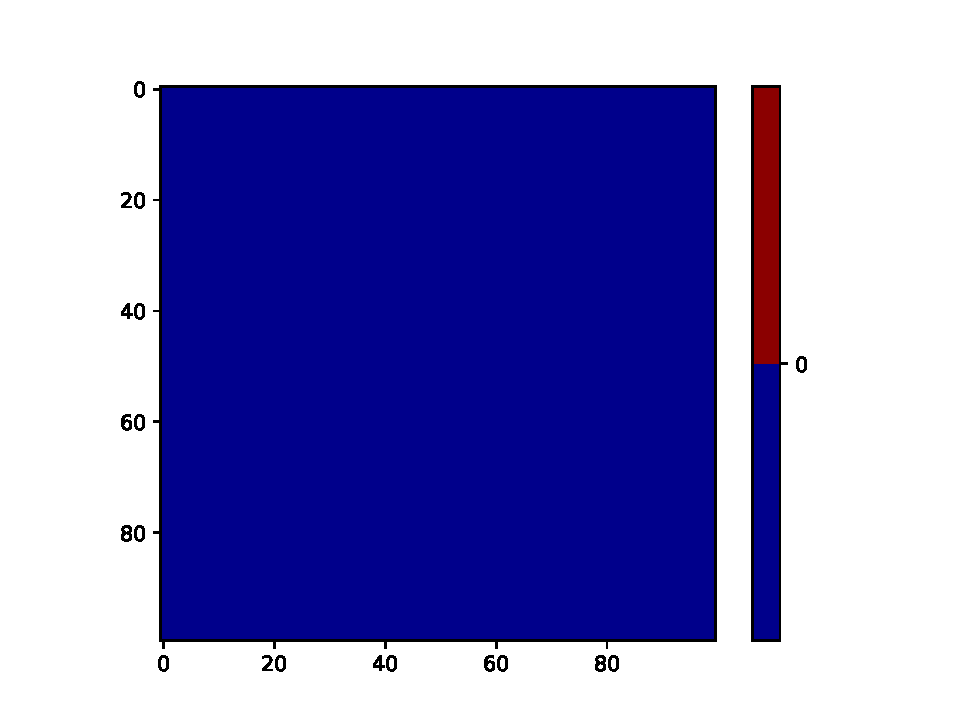
\includegraphics[width = 0.8\textwidth]{A2/build/1kbt-a-fest_anfang.pdf}
    \caption{Anfang}
  \end{subfigure}
  \begin{subfigure}{0.48\textwidth}
    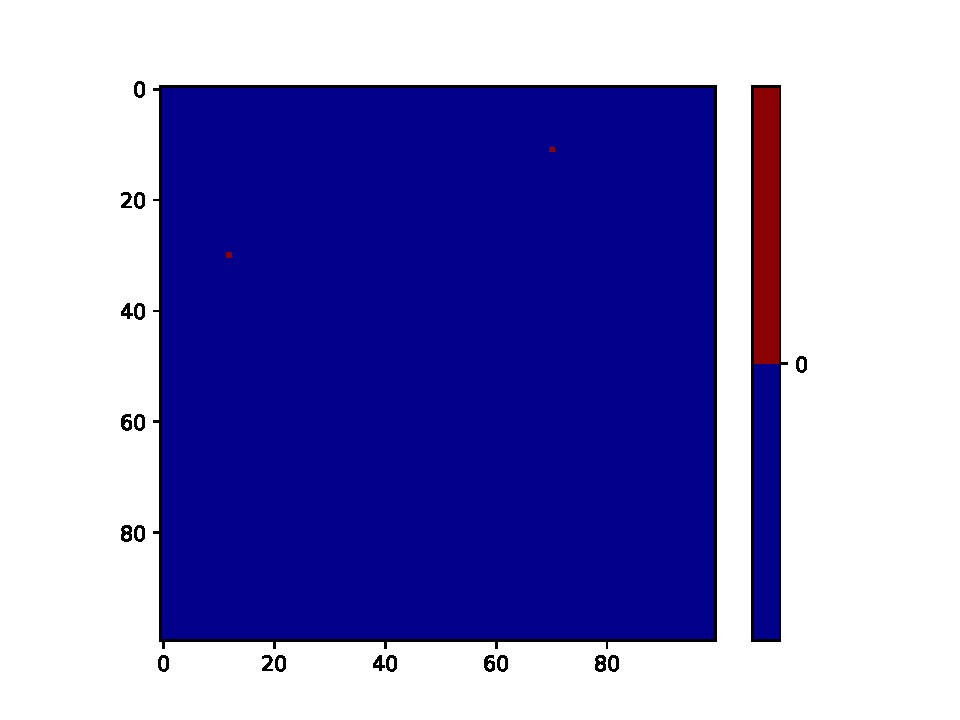
\includegraphics[width = 0.8\textwidth]{A2/build/1kbt-a-fest_ende.pdf}
    \caption{Ende}
  \end{subfigure}
  \caption{Momentaufnahme für feste Spins $k_B T =1$ am Anfang und Ende der Simulation. }
  \label{fig:fixOne}
\end{figure}

\begin{figure}
  \begin{subfigure}{0.48\textwidth}
    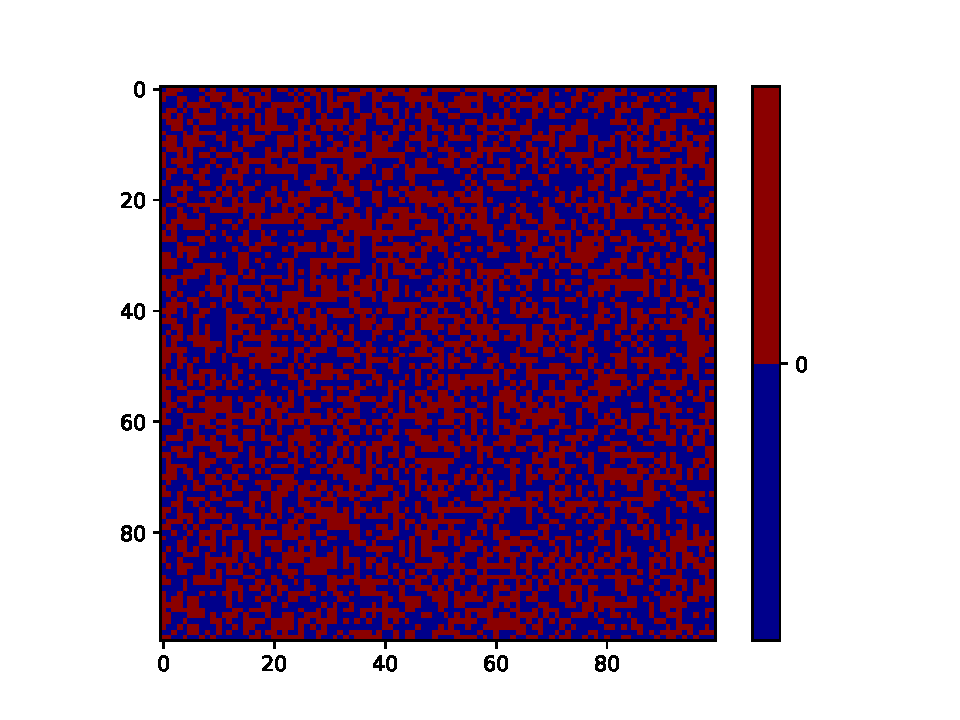
\includegraphics[width = 0.8\textwidth]{A2/build/1kbt-a-zufall_anfang.pdf}
    \caption{Anfang}
  \end{subfigure}
  \begin{subfigure}{0.48\textwidth}
    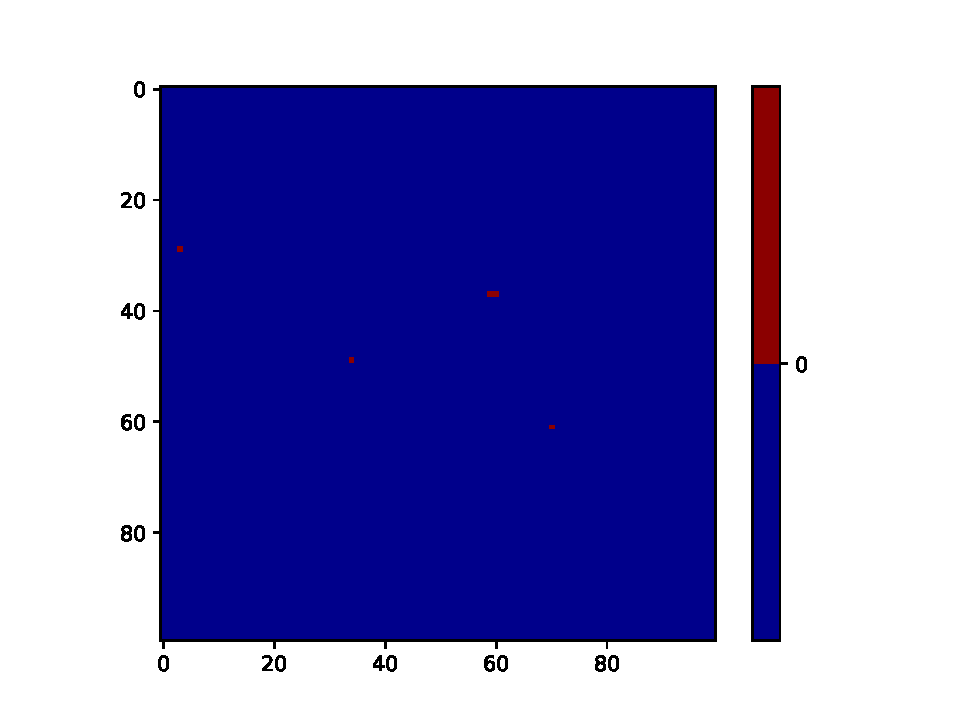
\includegraphics[width = 0.8\textwidth]{A2/build/1kbt-a-zufall_ende.pdf}
    \caption{Ende}
  \end{subfigure}
  \caption{Momentaufnahme für zufällige Spins mit $k_B T =1$ am Anfang und Ende der Simulation.}
  \label{fig:randomOne}
\end{figure}

\begin{figure}
  \begin{subfigure}{0.48\textwidth}
    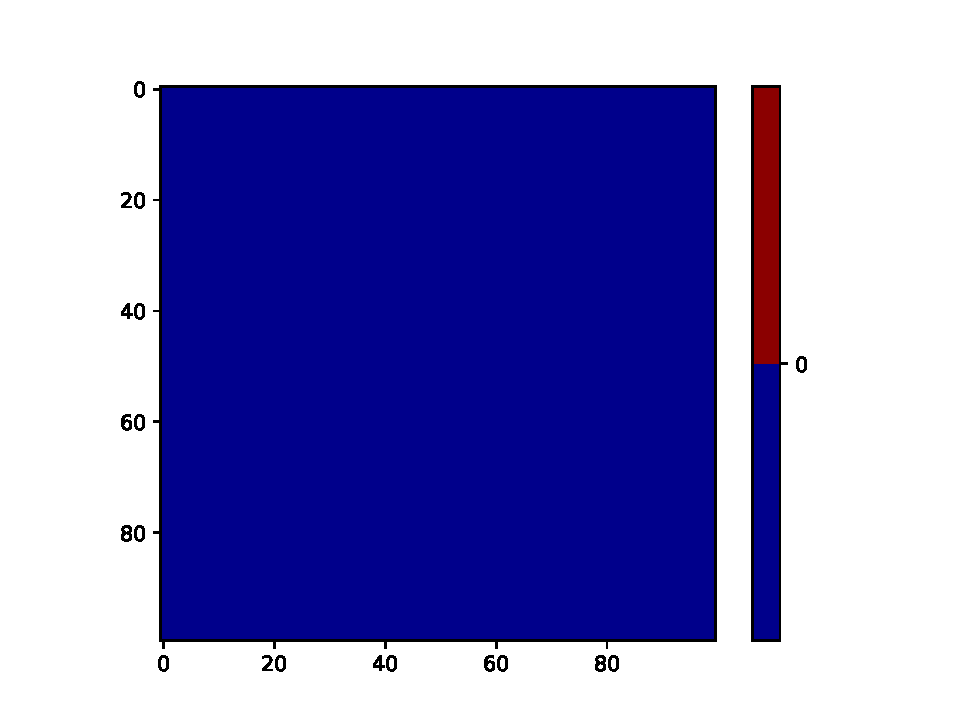
\includegraphics[width = 0.8\textwidth]{A2/build/3kbt-a-fest_anfang.pdf}
    \caption{Anfang}
  \end{subfigure}
  \begin{subfigure}{0.48\textwidth}
    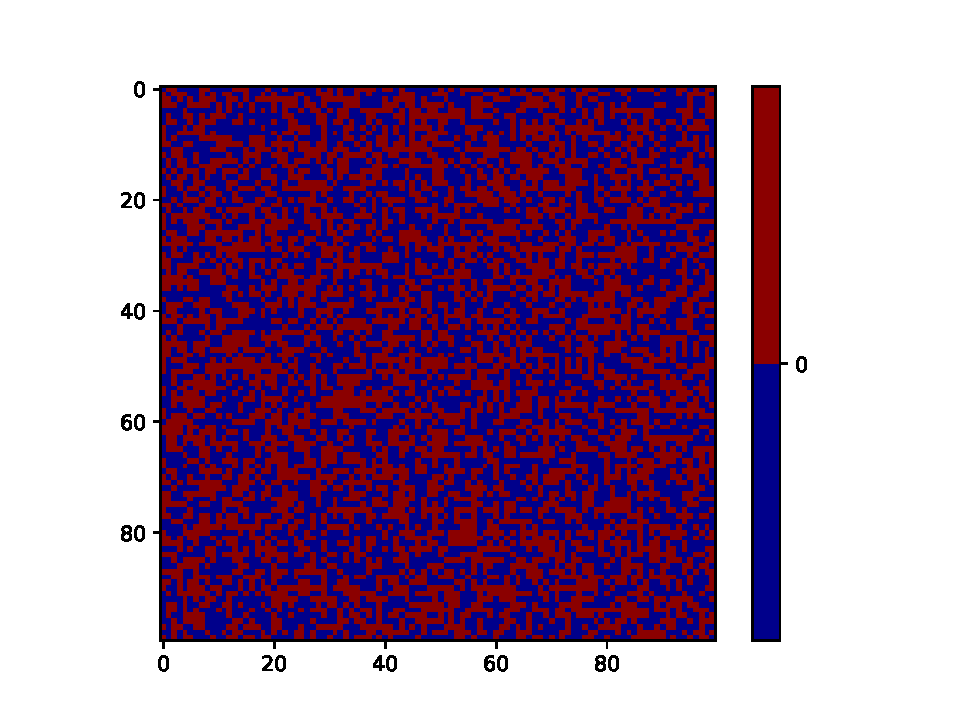
\includegraphics[width = 0.8\textwidth]{A2/build/3kbt-a-fest_ende.pdf}
    \caption{Ende}
  \end{subfigure}
  \caption{Momentaufnahme für feste Spins mit $k_B T = 3$ am Anfang und Ende der Simulation.}
  \label{fig:fixThree}
\end{figure}

\begin{figure}
  \begin{subfigure}{0.48\textwidth}
    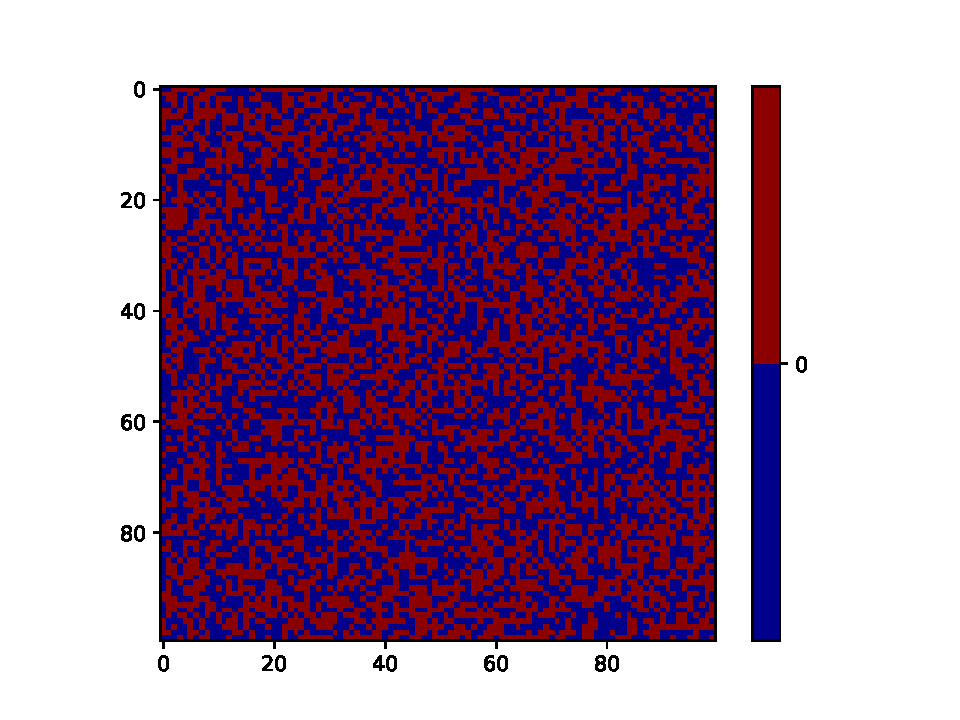
\includegraphics[width = 0.8\textwidth]{A2/build/3kbt-a-zufall_anfang.pdf}
    \caption{Anfang}
  \end{subfigure}
  \begin{subfigure}{0.48\textwidth}
    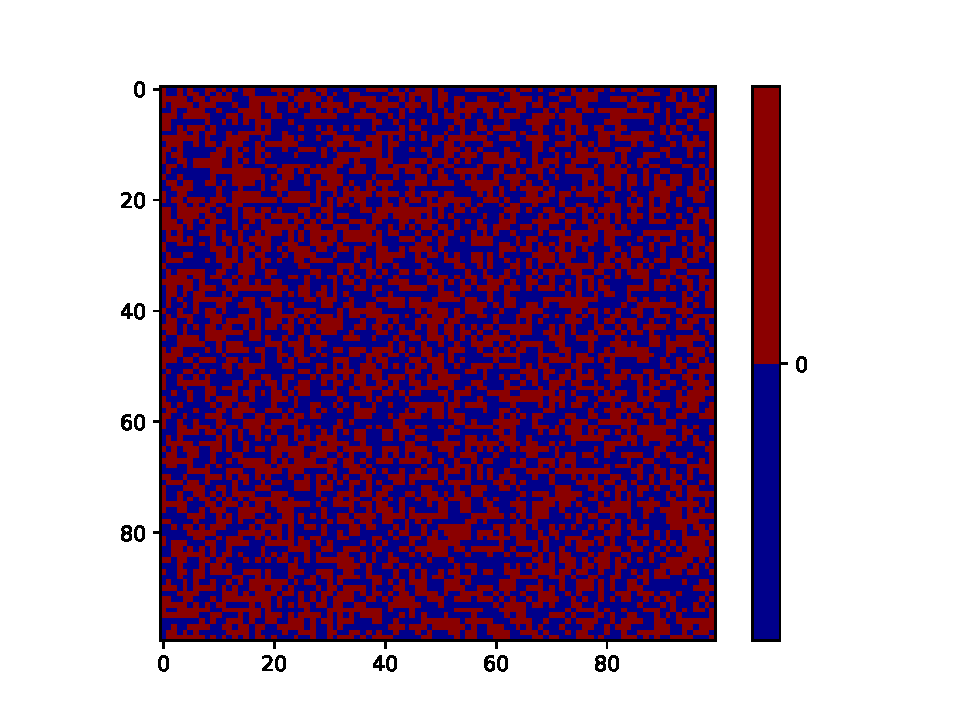
\includegraphics[width = 0.8\textwidth]{A2/build/3kbt-a-zufall_ende.pdf}
    \caption{Ende}
  \end{subfigure}
  \caption{Momentaufnahme für zufällige Spins mit $k_B T = 3$ am Anfang und Ende der Simulation.}
  \label{fig:randomThree}
\end{figure}

\subsection*{b)}
In Abbildung \ref{fig:b} ist die mittlere Energie pro Spin gegen die Simulationszeit $t$ aufgetragen. Dabei ist zu erkennen, dass verschiedene Startbedingungen zu unterschiedlichen Zuständen führen. Besonders auffällig sind dabei die Energien für $k_B T = 3$, die zu divergieren scheinen. Dies entspricht nicht unserer Erwartung  – wir erwarten, dass ich eine Äquilibrierung einstellt –, weshalb wir einen Fehler im Code vermuten, den wir leider nicht mehr finden konnten. 

\begin{figure}
  \centering
  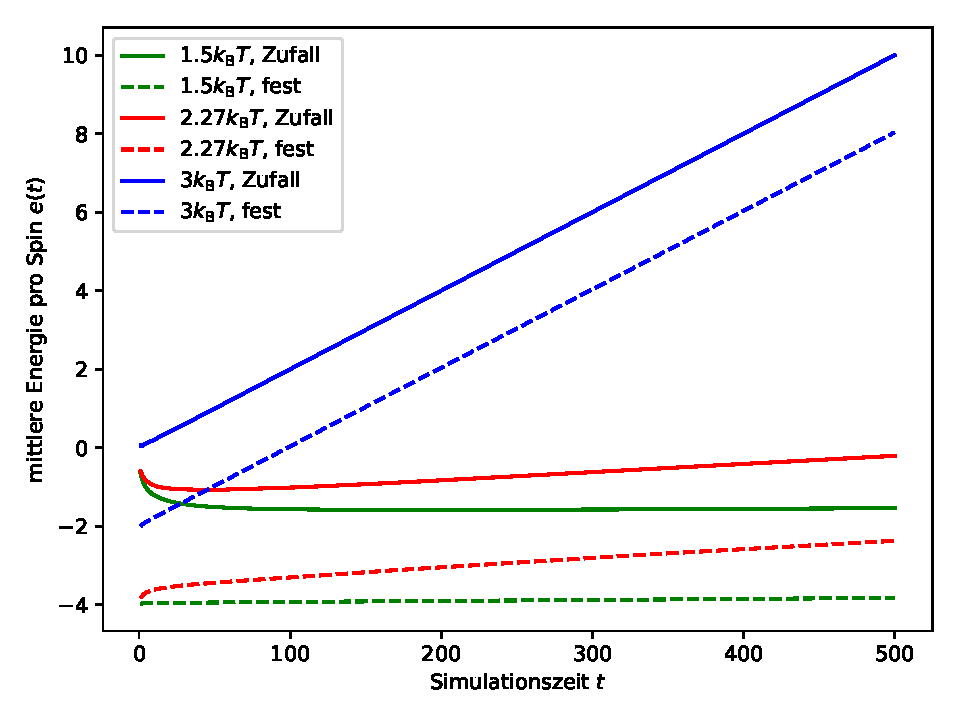
\includegraphics[width = 0.8\textwidth ]{A2/build/plot_b.pdf}
  \caption{Mittlere Energie pro Spin für die einzelnen Startbedingungen aufgetragen gegen die Zeit.}
  \label{fig:b}
\end{figure}
